\documentclass[compress]{beamer}
\setbeamercolor{normal text}{fg=black}
\setbeamercovered{transparent, still covered={\opaqueness<1->{0}}, again covered={\opaqueness<1->{30}}}
\beamertemplatesolidbackgroundcolor{white}
\usecolortheme[named=black]{structure}
\usepackage{caption}
\captionsetup{labelformat=empty}
\setbeamertemplate{navigation symbols}{}
%\usefonttheme{structurebold}
\usepackage{listings}
\usepackage{ulem}
\usepackage[scaled]{helvet}
\renewcommand*\familydefault{\sfdefault} %% Only if the base font of the document is to be sans serif
\usepackage[T1]{fontenc}
\usepackage{setspace}
%\usepackage{beamerthemesplit}
\usepackage{graphics}
\usepackage{hyperref}
\usepackage{graphicx}
\usepackage{verbatim}
\usepackage{amssymb}
\usepackage{wrapfig}
\usefonttheme[onlymath]{serif}
\usepackage{cmbright}

\def\labelitemi{\textemdash}
\setbeamertemplate{frametitle}{
	\begin{centering}
		\vskip15pt
		\insertframetitle
		\par
	\end{centering}
}
\title[domains]{\\ \vspace{10mm} domain knowledge}
\author[Sood and Laohaprapanon]{gaurav and suriyan}
  \large
\date[2020]{}
\subject{Paper}
\begin{document}
\newcommand{\multilineR}[1]{\begin{tabular}[b]{@{}r@{}}#1\end{tabular}}
\newcommand{\multilineL}[1]{\begin{tabular}[b]{@{}l@{}}#1\end{tabular}}
\newcommand{\multilineC}[1]{\begin{tabular}[b]{@{}c@{}}#1\end{tabular}}
\newcommand{\indep}{\rotatebox[origin=c]{90}{$\models$}}
\newenvironment{large_enum}{
\Large
\begin{itemize}
  \setlength{\itemsep}{7pt}
  \setlength{\parskip}{0pt}
  \setlength{\parsep}{0pt}
}{\end{itemize}}

\begin{comment}

setwd(paste0(githubdir, "domain_knowledge/present/"))
tools::texi2dvi("domain_knowledge.tex", pdf = TRUE, clean = TRUE)
setwd(basedir)

\end{comment}
  \frame
  {
    \titlepage
  }

\frame{

\Large{Why predict the category of content hosted by a domain?}
\pause

\begin{large_enum}
	\item[-]<2>malware and phishing
	\item[-]<3>adult content
	\item[-]<4->personalization
		\begin{itemize}
			\item[-]<5>you can have your \textit{cookie} and eat it too!
		\end{itemize}
\end{large_enum}
}

\frame{

\Large{But if we were to learn from domain names, how would we?}
\pause

\begin{large_enum}
	\item[-]<2>manual labeling---\texttt{PhishTank, DMOZ}, etc.
	\item[-]<3>meta tags---self reports
	\item[-]<4>metadata: how the pages are laid out, how many images, etc.
	\item[-]<5>content understanding: text, images, etc.
	\item[-]<6->\only<6>{signal in the url}\only<7>{\alert{signal in the url}}
	\end{large_enum}
}

\frame{

\Large{Considerations}
\pause

\begin{large_enum}
	\item[-]<2-3>computational burden, speed\\
			\only<3->{\normalsize{$>$ 2B domains}}
	\item[-]<3>privacy
	\item[-]<4>accuracy
	\end{large_enum}
}

\frame{

\Large{Intuition}

\begin{large_enum}
  \item[-]<2-3> Patterns in names. \\
		\only<3->{\normalsize{words like \textit{xxx, porn, adult, sex} etc. common in domains carrying pornographic content}}
  \item[-]<4-5>$>$ 200 \texttt{PhishTank} URLs have the word \textit{paypal} in them. \\
			\only<5>{\normalsize{compare with Alexa 1M to build classifiers that can tell those apart}}
\end{large_enum}

}

\frame{
\Large{How to Classify Text\\}

\begin{large_enum}
   \item[-]<1-5> Text $\leadsto$ Embeddings $\leadsto$ Classifier
		\begin{enumerate}
			\item[-]<2-> Embeddings leverage the adage:\\
						  You are the company you keep.
			\item[-]<3-> Use a large corpus
			\item[-]<4-> Learn the context well
			\item[-]<5-> Preserve tens of hundreds of vectors and pass them to a model
	    \end{enumerate}

	\item[-]<6->In Our Case:
		\begin{enumerate}
			\item[-]<7-> Embeddings of common bi-chars
			\item[-]<8-> LSTM
		\end{enumerate}
	\end{large_enum}
}

\frame{

\begin{figure}
  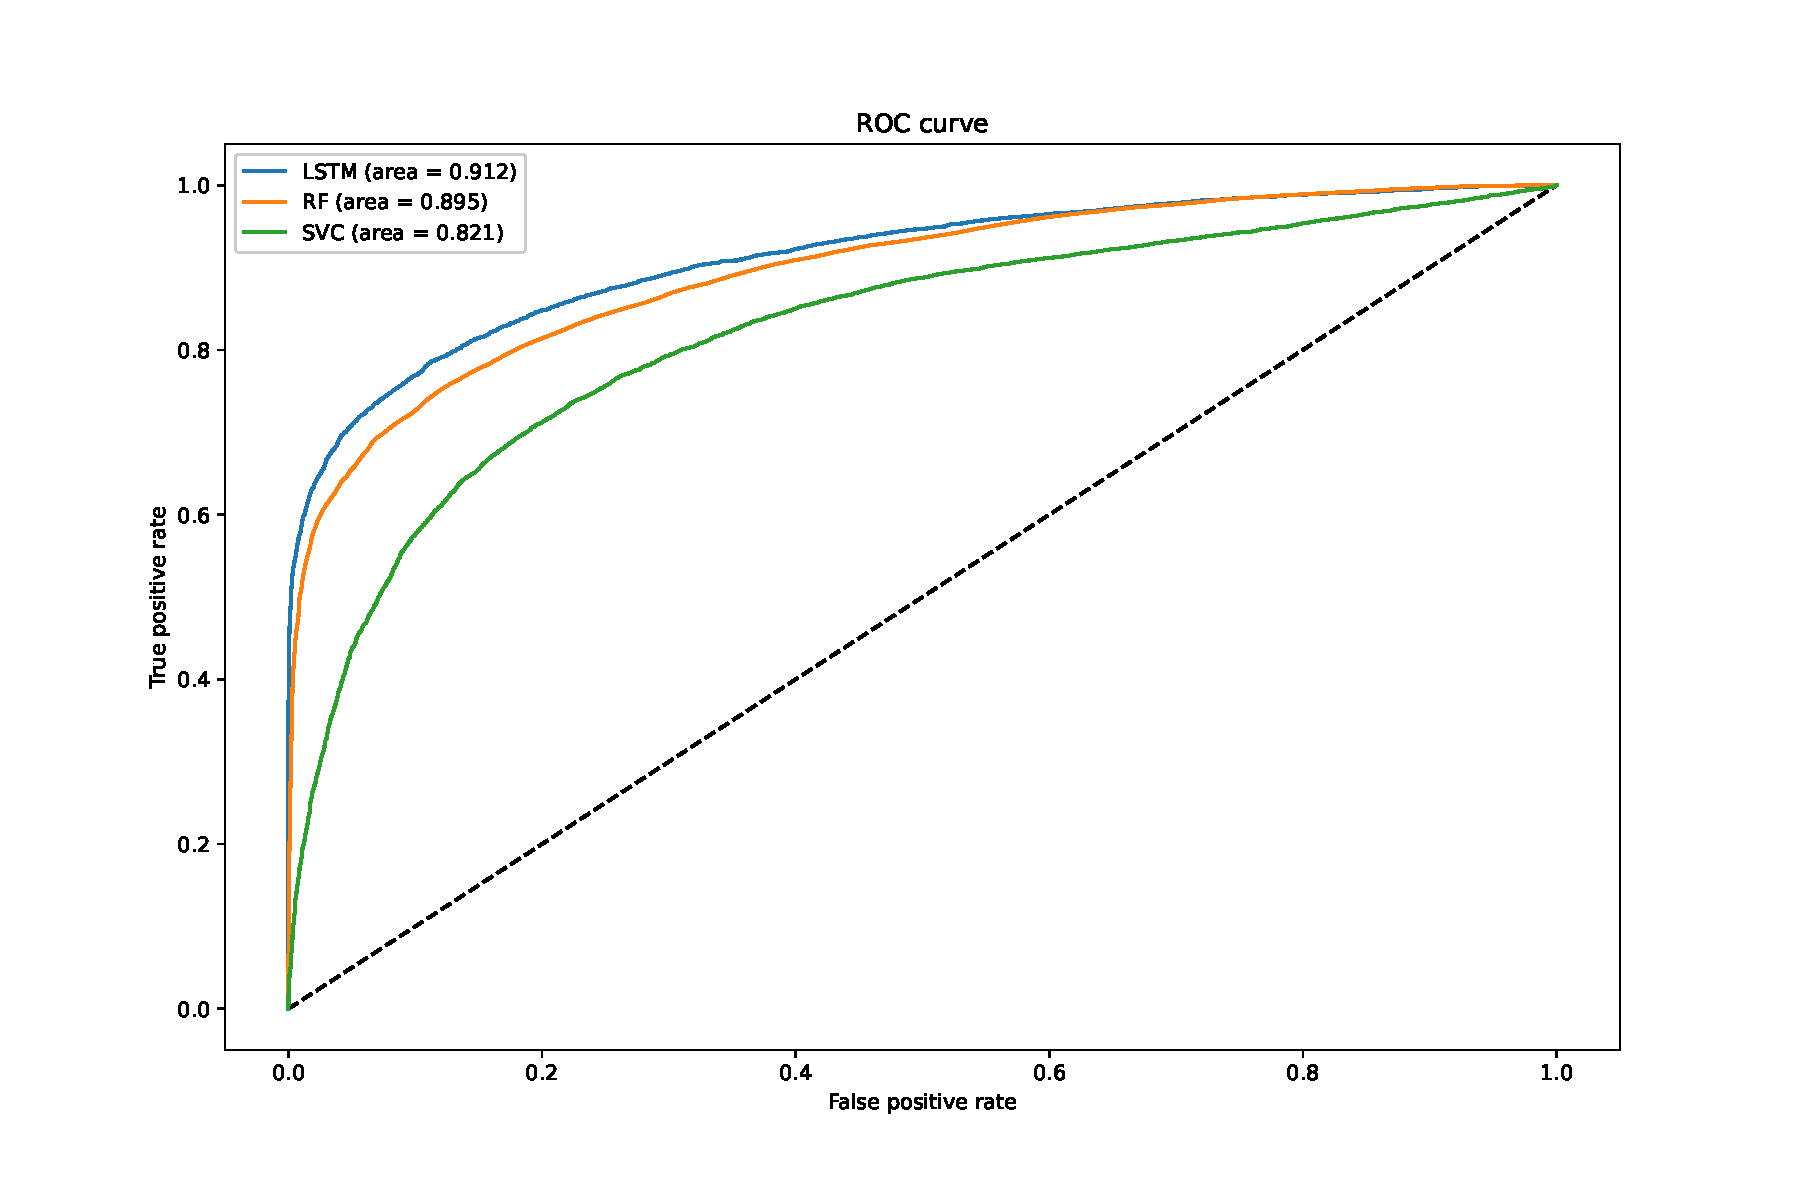
\includegraphics[width=\linewidth]{../figs/roc-phish-2017-lstm-rf-svc.pdf}
  \caption{PhishTank}
\end{figure}
}

\frame{

\only<1->{\Large{Application}}

\begin{large_enum}
  \item[-]<2> Are disadvantaged people most at risk online?
\end{large_enum}

\only<4->{\Large{Data}}
\begin{large_enum}
  \item[-]<5> comScore panel
  \item[-]<6> domain level data for a machine in a household + household attributes
\end{large_enum}
}

\frame{

\only<1->{\Large{Concerns}}

\begin{large_enum}
  \item[-]<2>Domain $!=$ URL
  \item[-]<3>Net error is a function of FP - FN.
	\item[-]<4>The larger the number of domains, the larger the error in their score
	\item[-]<5>Visits are right-skewed. Errors in the right tail are very costly.
\end{large_enum}

\only<6->{\Large{Solutions}}

\begin{large_enum}
  \item[-]<7>Calibration $\leadsto FP = FN$ locally
	\item[-]<8>Using curated lists (manual coding) for popular domains
\end{large_enum}

}

\frame{
\Large{\only<1>{The better educated visit phishing/malware domains most often}}
\only<2->{


\begin{figure}
  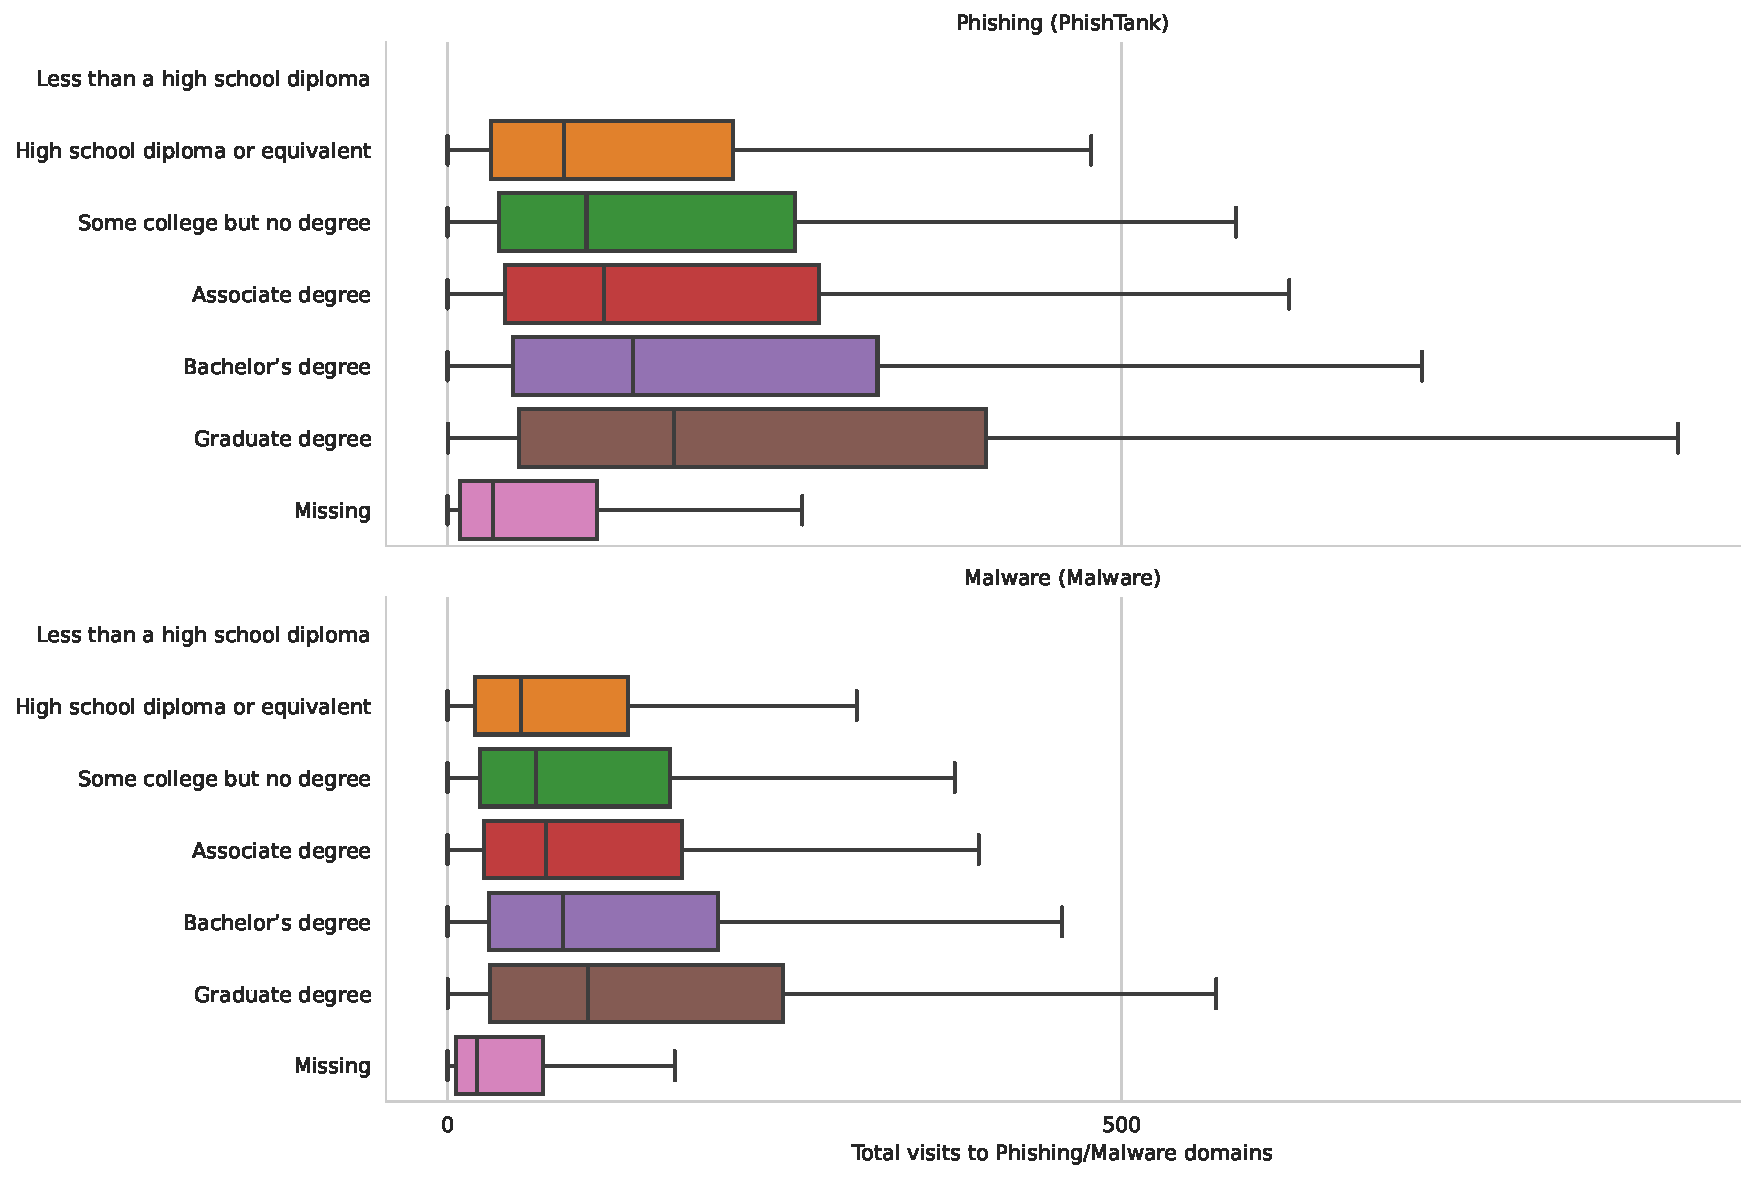
\includegraphics[width=\linewidth]{../figs/total_visits_phishing_malware_educ.pdf}
  \caption{Visits to phishing/malware domains}
\end{figure}

}
}

\frame{
\Large{\only<1>{But the better educated don't choose worse}}
\only<2->{


\begin{figure}
  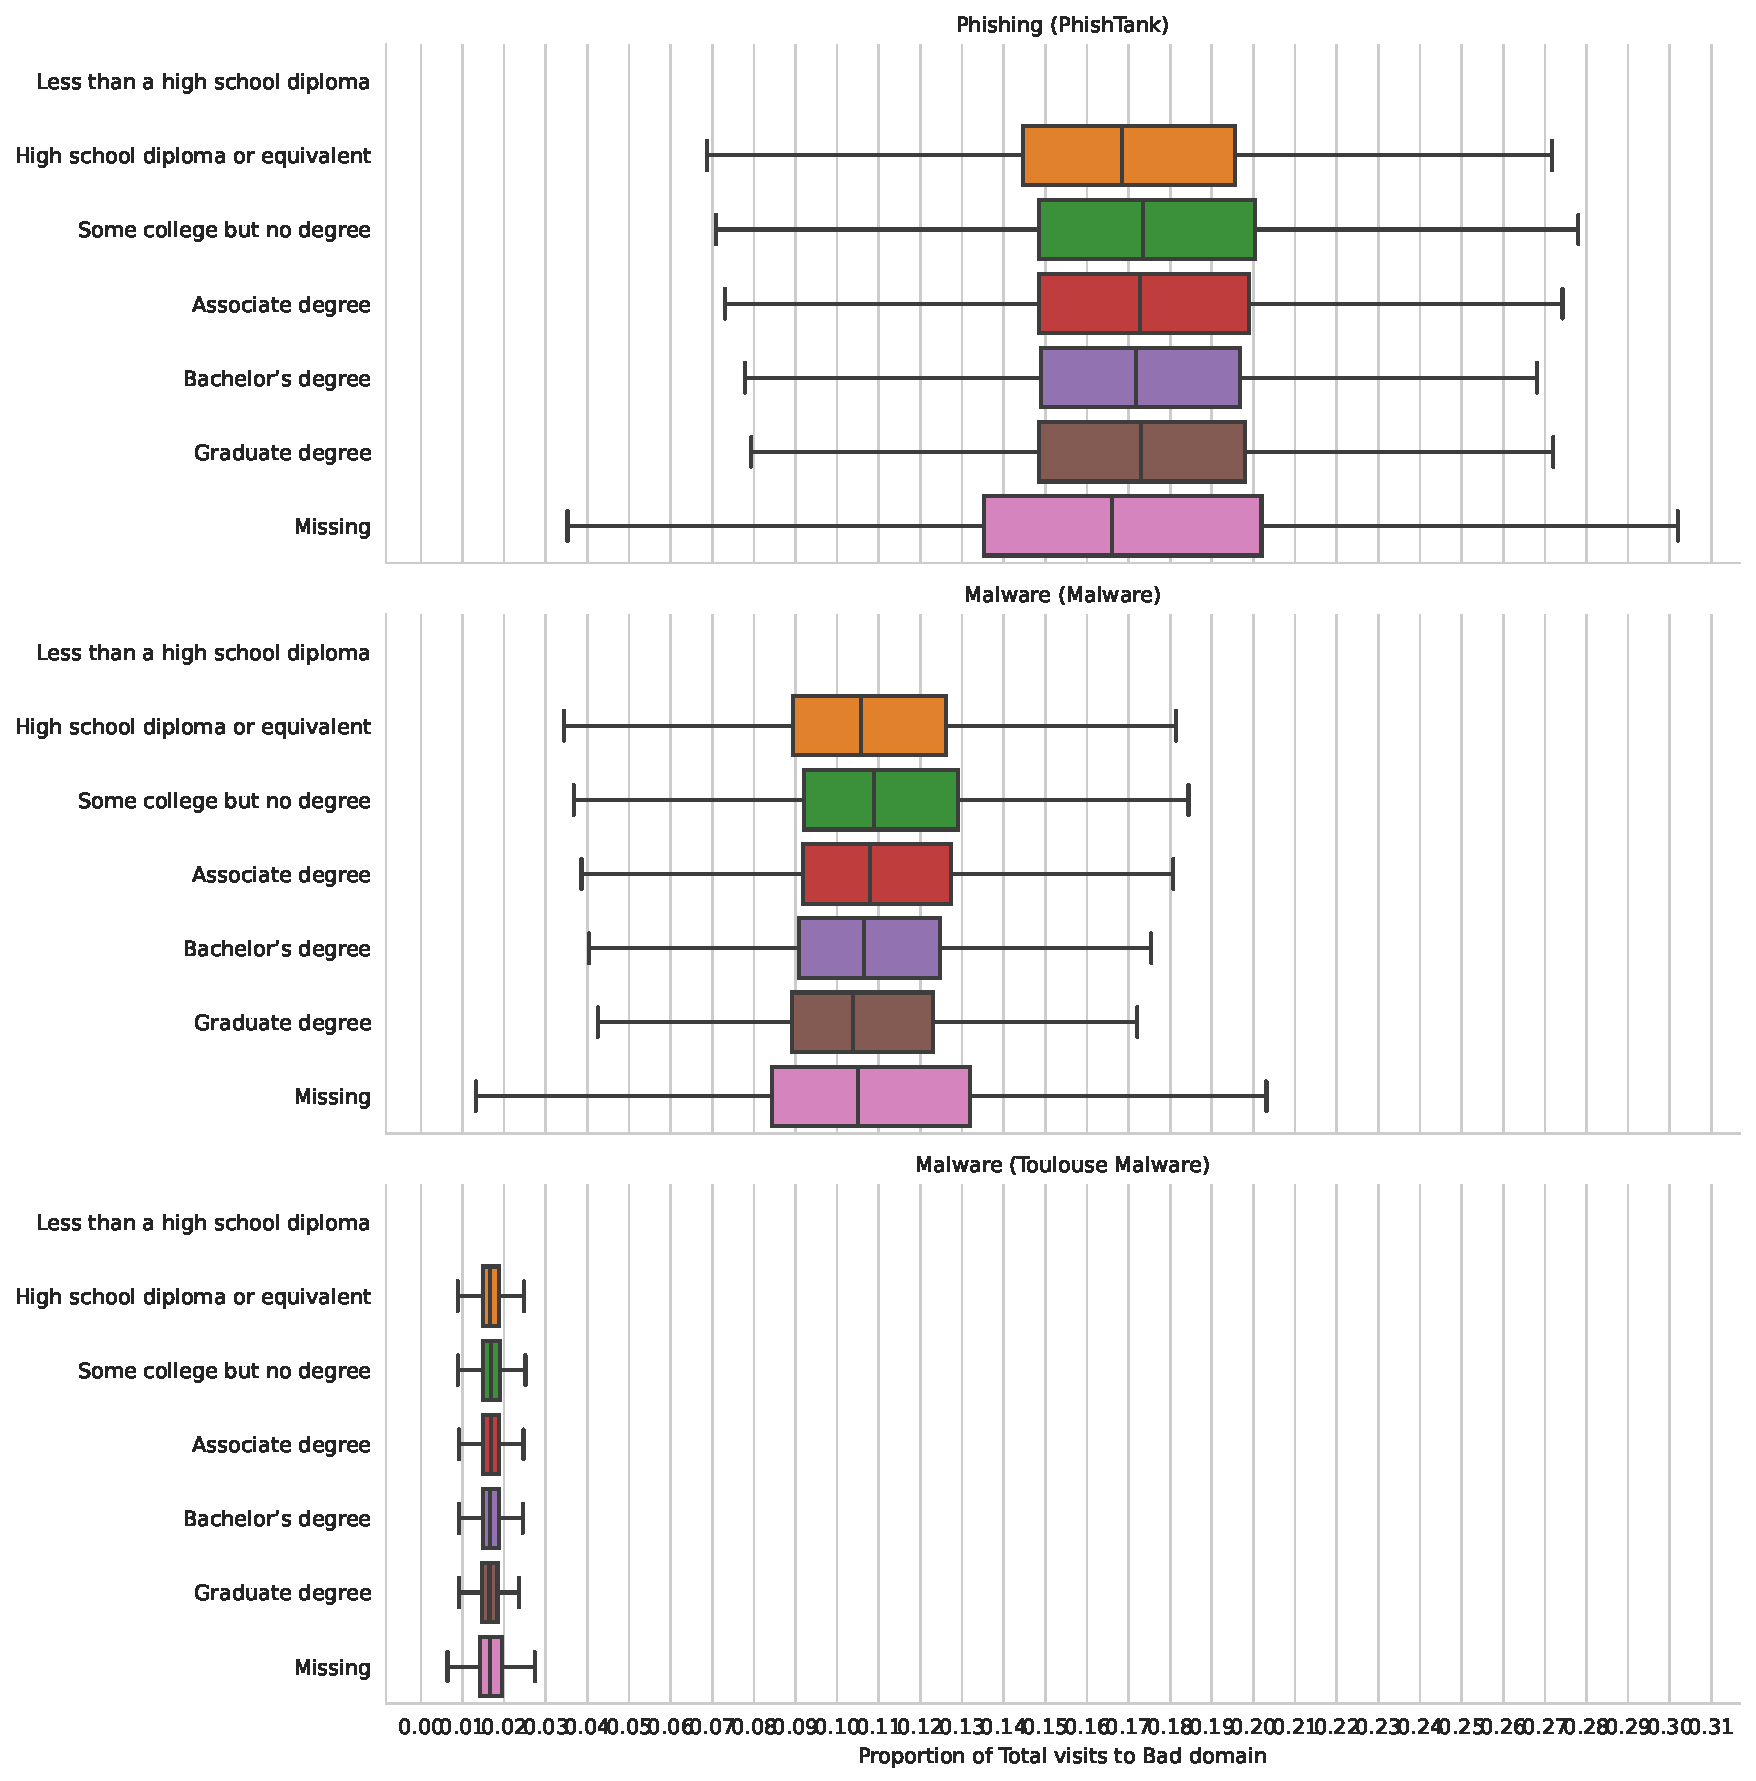
\includegraphics[width=.7\linewidth]{../figs/prop_total_visits_phishing_malware_tl_educ.pdf}
  \caption{Proportion of visits to phishing/malware domains}
\end{figure}

}
}


\end{document}
